\documentclass[a4paper,titlepage,oneside,12pt]{amsart} %amsart
\usepackage{graphicx}
\usepackage{hyperref}
%\usepackage{geometry} % see geometry.pdf on how to lay out the page. There's lots.
\usepackage[margin=1.3in]{geometry}
\geometry{a4paper} % or letter or a5paper or ... etc
% \geometry{landscape} % rotated page geometry
\usepackage{ifthen}

% See the ``Article customise'' template for come common customisations
\usepackage[usenames,dvipsnames]{color}

\definecolor{lightgray}{RGB}{245, 245, 245}
\definecolor{bkblue}{RGB}{18, 47, 76}
\definecolor{bklightblue}{RGB}{102, 131, 158}
\definecolor{mygreen}{rgb}{0,0.6,0}
\definecolor{orange}{RGB}{255,153,0}

\usepackage{opensans}
\usepackage{setspace}
\usepackage{booktabs} \newcommand{\ra}[1]{\renewcommand{\arraystretch}{#1}}

\usepackage{color}
\newcommand{\todo}[1]{\colorbox{yellow}{#1}}
\newcommand{\toread}[1]{{\color{bklightblue} #1}}

\usepackage{listings}
\lstset{ %
language=C,                % choose the language of the code
basicstyle=\footnotesize,       % the size of the fonts that are used for the code
%numbers=left,                   % where to put the line-numbers
%numberstyle=\footnotesize,      % the size of the fonts that are used for the line-numbers
%stepnumber=1,                   % the step between two line-numbers. If it is 1 each line will be numbered
%numbersep=5pt,                  % how far the line-numbers are from the code
backgroundcolor=\color{lightgray},  % choose the background color. You must add \usepackage{color}
showspaces=false,               % show spaces adding particular underscores
showstringspaces=false,         % underline spaces within strings
showtabs=false,                 % show tabs within strings adding particular underscores
frame=single,           % adds a frame around the code
framerule=0.2pt,
tabsize=2,          % sets default tabsize to 2 spaces
captionpos=b,           % sets the caption-position to bottom
breaklines=true,        % sets automatic line breaking
breakatwhitespace=false,    % sets if automatic breaks should only happen at whitespace
escapeinside={\%*}{*)},          % if you want to add a comment within your code
belowcaptionskip=5em,
belowskip=1em,
aboveskip=1.8em,
commentstyle=\itshape\color{mygreen},
keywordstyle=\bfseries\color{black},
identifierstyle=\color{black},
stringstyle=\color{blue},
morekeywords={*, }
}

\newcommand{\versionNr}{0.1}
\newcommand{\authorMila}{Dr. sc. Milanka Ringwald}
\newcommand{\authorMatthias}{Dr. sc. Matthias Ringwald}
\newcommand{\bkContact}{\href{contact@bluekitchen-gmbh.com}{contact@bluekitchen-gmbh.com}}
\newcommand{\barWidth}{0.3cm}

\makeatletter
\renewcommand{\maketitle}{
  \begin{titlepage}
    \fosfamily
    \begin{center}
    \begin{minipage}[b]{\textwidth}
        \begin{minipage}[b]{.1\textwidth}
            \color{bkblue}\rule{\barWidth{}}{22cm}
        \end{minipage}
        \hfill\begin{minipage}[b]{.8\textwidth}\begin{flushright}
            {\color{bkblue}VERSION \versionNr{} \\
            \today \\}
            \vspace*{7.5cm}
            \hfill
\includegraphics[width=0.95\textwidth]{../../../docs/manual/picts/bklogo.pdf}
            \vspace*{1.5cm}
            \begin{spacing}{2} 
                {\huge \color{bkblue} \@title} \\ 
                {\Large \color{bklightblue} Getting Started}   
            \end{spacing} 
            \vspace*{1.5cm}
            {\color{bkblue}\large \authorMila \\
            \large \authorMatthias \\
            \large \bkContact\\ }
        \end{flushright}\end{minipage}
        \vfill
        \begin{minipage}[b]{\textwidth}
            \color{bklightblue}\rule{\barWidth{}}{\barWidth{}}
        \end{minipage}
    \end{minipage}

    
    \end{center}
  \end{titlepage}
}
\makeatother

\title[] {BTstack for RugGear/MediaTek Chipsets} 
\author{Copyright \copyright  2014 BlueKitchen GmbH}

%%% BEGIN DOCUMENT
\begin{document}

\maketitle

\tableofcontents
\pagebreak

\newcommand{\urlfoot}[2]{\href{#1}{{\color{blue} #2}}\footnote{#1}}
\newcommand{\BTstack}{\urlfoot{http://bluekitchen-gmbh.com/btstack}{BTstack}{}}
\newcommand{\CydiaImpactor}{\urlfoot{http://www.cydiaimpactor.com}{Cydia Impactor}{}}
\newcommand{\CydiaImpactorURL}{\href{http://www.cydiaimpactor.com}{\color{blue} Cydia Impactor}}

\newcommand{\ADT}{\urlfoot{http://developer.android.com/tools/index.html}{Android Developer Tools}{}}
\newcommand{\nio}{\urlfoot{https://www.bluenio.com/products/accessories/niotag}{nio Tag}{}}
\newcommand{\PacketLogger}{\urlfoot{http://adcdownload.apple.com/Developer\_Tools/hardware\_io\_tools\_for\_xcode\_\_june\_2014/hardwareiotools\_june\_2014.dmg}{PacketLogger}{}}
\newcommand{\Wireshark}{\urlfoot{http://www.wireshark.org}{Wireshark}{}}
\newcommand{\Cygwin}{\urlfoot{https://www.cygwin.com}{Cygwin}{}}
\newcommand{\MSYS}{\urlfoot{www.mingw.org/wiki/msys}{MSYS}{}}
\newcommand{\adb}{\urlfoot{http://developer.android.com/tools/help/adb.html}{Android Debug Bridge}{}}

This documents describes how \BTstack{} can be installed and used on RugGear devices with MediaTek chipset. It also presents measurements of the reception of Advertising reports from a remote devices, e.g. beacons or peripherals, as this is the crucial step for discovering and connecting to them.

\section{Hardware Setup} 
To install BTstack on a RugGear mobile phone, connect the RugGear device to a Mac or Linux system using a micro USB cable. The installation might also work on Windows with \Cygwin{} and/or \MSYS{} installed. The RugGear device is connected to an USB port during setup and development.

\section{General Tools}

\begin{itemize}
\item \CydiaImpactor{} to get root access.
\item Google's \ADT{} (ADT) to develop an Android LE Client. 
\item The \adb{} (adb) to communicate with a connected Android device via a command line. It comes as a part of the Android Developer Tools.
\item Apple's \PacketLogger{} (available to the registered developers as part of the Hardware IO Tools for Xcode download) or \Wireshark{} to look and analyze Bluetooth packet logs.
\item Some LE devices that send Advertising reports to test your LE Client. Here, we used the \nio{} and a BTstack-based LE Peripheral on a desktop machine using the BCM20702A0 module.
\end{itemize}

\section{Rooting the RugGear Device}
There are various ways to root an Android device. We recommend the \CydiaImpactorURL{} tool. It is available for all major platforms, it works with most Android devices and it comes from a trustworthy source\footnote{It was created by Jay Freeman, who has supporting the use iOS devices outside of Apple's walled garden since the device came out}. 

To root the device, start Impactor, and press the "Start" button as shown in Fig.\ref{fig:cydiaimpactor} 

\begin{figure}[htbp]
\begin{center}
 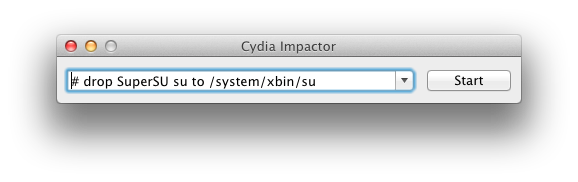
\includegraphics[width=\textwidth]{picts/cydiaimpactor.png} 
\caption{Cydia Impactor running on OS X.}
\label{fig:cydiaimpactor}
\end{center}
\end{figure}

\section{Installing BTstack on RugGear devices with MediaTek Chipsets}

First, extract the provided \path{btstack-android-mtk-VERSION.tar.gz} archive. Please make sure that the path to the extracted archive does not contain spaces as the installer may fail in this case. Then, start the provided \path{./installer.sh} in the \path{mtk} folder. This should look similar to this listing.

\begin{lstlisting}
$ mkdir btstack
$ tar -zxvf btstack-android-mtk.tar.gz -C btstack
$ ls btstack
java	mtk
$ cd btstack/mtk
$ ./installer.sh
BTstack Installer for RugGear/Mediatek devices
from: .
- /system mounted as read/write
- stopping Bluetooth daemon
- transfer files to device
9192 KB/s (279736 bytes in 0.029s)
2949 KB/s (6188 bytes in 0.002s)
7753 KB/s (62360 bytes in 0.007s)
4184 KB/s (11316 bytes in 0.002s)
3201 KB/s (6592 bytes in 0.002s)
5348 KB/s (11720 bytes in 0.002s)
- put files in place
- start BTstack daemon
DONE
\end{lstlisting}

If BTstack was installed properly, we can have a look at its packet log.

\begin{lstlisting}
$ make hci_dump
killall PacketLogger
adb shell su root chmod 666 /data/btstack/hci_dump.pklg
adb pull /data/btstack/hci_dump.pklg 2> /dev/null
open hci_dump.pklg
\end{lstlisting}

The \path{make} \path{hci_dump} command assumes that the underlying system is OS X and that PacketLogger is already running. The two\path{adb} commands, shown in the following Listing, are used to fetch the packet log (hci\_dump.pklg) and it can be run on any platform. Wireshark can then be used to open the packet log.

\begin{lstlisting}
$ adb shell su root chmod 666 /data/btstack/hci_dump.pklg
$ adb pull /data/btstack/hci_dump.pklg 2> /dev/null
\end{lstlisting}

The initial packet log should look like in Figure \ref{fig:firstLog}.

\begin{figure}[htbp]
\begin{center}
 \includegraphics[width=\textwidth]{picts/ruggear_initial_hci_dump.pdf} 
\caption{hci\_dump.pklg right after BTstack daemon was installed.}
\label{fig:firstLog}
\end{center}
\end{figure}

\section{Running the First Example}

As first, make sure that BTstack was installed properly and it is running, i.e. by checking the packet log as explained in the previous section. Now, let's do an LE Scan using a test program written in C against libBTstack.

\begin{lstlisting}
$ adb shell
$ le_scan
le_scan started
- connecting to BTstack Daemon
- connected
- send power on
- btstack state 1
- btstack state 2
- start LE scan
- ADV: 3E 0F 02 01 00 01 F2 01 8F 45 16 66 03 02 01 1A B3
\end{lstlisting}

The \path{le\_scan} just dumps the data of each received advertisement. It uses the default parameters used by iOS, which are scan window 30 ms, scan interval 300 ms. More on these parameters is in Section \ref{ss:measurements}. The packet log looks like in Figure \ref{fig:leScan}.

\begin{figure}[htbp]
\begin{center}
 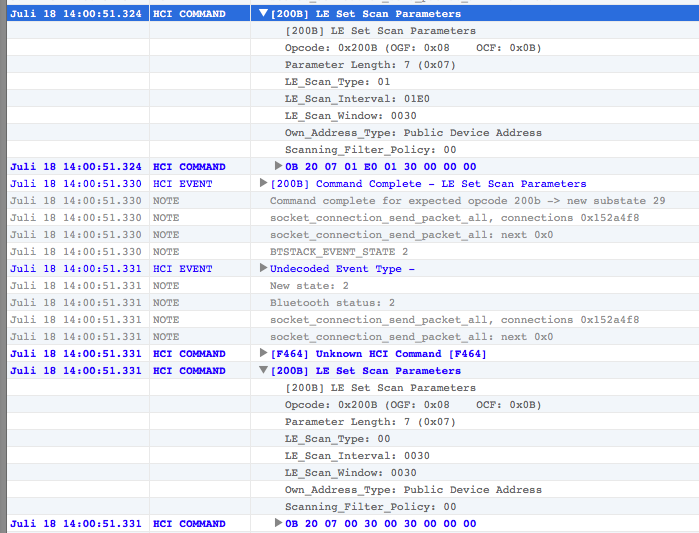
\includegraphics[width=\textwidth]{picts/scan_parameters_hci_dump.png} 
\caption{HCI dump of the le\_scan program.}
\label{fig:leScan}
\end{center}
\end{figure}

\section{BTstack Java API}

BTstack on RugGear/MediaTek provides its own Bluetooth stack and its own interface for using it. While BTstack has been certified for Classic SPP and LE Peripheral, it does not provide a complete Java API for this. At the moment, the functionality to turn Bluetooth on/off, scan for LE devices, connect, and make use of Services and Characteristics is provided. This covers the use of BTstack as LE Central. Please note that the Security Manager is not implemented yet. Use of the Security Manager is necessary when devices require explicit pairing before some services can be used.

 The Java classes that make up the BTstack API  are split into three folders. Please add all of them to your Android Java project:
 
 \begin{enumerate}
\item \path{java/src} - main code for BTstack client, i.e., socket communication with BTstack server that runs as a daemon.
\item \path{java/android} - Android specific Client/Server communication.
\item \path{java/gen} -  code for available commands and events, auto-generated from the BTstack C source.
\end{enumerate}

\subsection{BTstack GATT Client for Android example}
More documentation on the Java API is needed. For now, please have a look at the Anrdoid example in \path{java/example/com/bluekitchen/GATTClientTest.java}. It connects to BTstack Server and turns Bluetooth on. On success, it starts an LE Scan for devices. When it finds a device, it connects to it and queries the available Services. Then, it requests the list of Characteristics for the first service. Finally, it performs some read/write operations on the found Characteristics.

BTstack server runs as a daemon. In the event of a crash, the Java client will get notified and can restart the daemon, to provide a continuous use of the Bluetooth services.

\section{BCM20702A0 and RugGear RG500 Reception of Advertisements}
\label{ss:measurements}

During the first tests of BTstack on RugGear/MediaTek, we have seen that it receives less Advertisements than other devices.

Advertisements serve three main purposes:
\begin{enumerate}
\item They provide information that a particular device is in range and turned on.
\item They can provide some information without connecting to a particular device (e.g. its name, provided services, or even manufacturer specific data).
\item They allow to connect to a particular device, i.e., an LE device listens for incoming connection requests only a short moment after sending an Advertisement (to save energy).
\end{enumerate}

A setup with one device that sends Advertisements and one device that receives them, can be completely described by three parameters: 
\begin{enumerate}
\item the \emph{Advertisement Interval} - the period between two consecutive Advertisements being sent.
\item the \emph{Scan Interval} - it determines how frequent the receiving device listens for Advertisements.
\item the \emph{Scan Window} - the time window in which the receiving device listens for Advertisements.
\end{enumerate}

\subsection{Setup} To evaluate the MediaTek Bluetooth chipsets used in the RugGear RG500, we compared them to a common Bluetooth USB Dual-Mode Dongle that uses the Broadcom BCM20702A0. We used two LE Peripherals. As the first LE Peripheral, we setup another device with the BCM20702A0 and configured it to advertise every 30 ms. This is very often, but it helps to establish how good Advertisements are received, if they occur frequently. As a second more real-world example, we used the nio Tag without further configuration. Based on the measured results, the nio Tag advertises roughly every second. 

We measured two cases: 
\begin{enumerate}
\item continuous scanning (Scan Window 30ms, Scan Interval 30ms),
\item intermittent scanning (Scan Window 30ms, Scan Interval 300ms) as performed by iOS.
\end{enumerate}

\subsection{Process}
For the continuous and intermittent scanning measurements on the RugGear, we used the \path{le_scan} test. We let it run for 15 minutes in continuous, and then 15 min in intermittent scanning setup. For each of the two measurement, we retrieved the packet logs from the device.  We processed it an analyzed it using two Python scripts \path{process_scan.py} and \path{plot_scan.py}. The measurements with the BCM module have been carried out with the GATT Browser example of BTstack on OS. Hence, we have up to four experiments for each setup:
\begin{itemize}
\item BCM/BCM - BCM20702A0 receives Advertisements from second BCM 20702A0 module 
\item BCM/nio - BCM20702A0 receives Advertisements from nio tag
\item RugGear/BCM - RugGear RG500 receives Advertisements from BCM 20702A0 module
\item RugGear/nio - RugGear RG500 receives Advertisements from nio tag 
\end{itemize}

\subsection{Measurements with continuous scanning}
For this experiment with set the Scan Interval to 30 ms and the Scan Windows to 30 ms, which translates to continuous scanning.

The plot in Figure \ref{fig:accumulatedAds} shows how many Advertisements have been received for both receivers from the two senders. In the BCM/BCM combination, 27 out of max 33 (1s /30 ms) Advertisements have been received. On the RugGear device, only about 1 in 15 Advertisements have been received.

Figure \ref{fig:delayHist} shows the distribution of the time between two received Advertisements over the full range.
 
All setups but the RugGear vs. nio Tag, received an Advertisement every second, which is sufficient for most interactive applications. We further analyzed the RugGear vs. nio Tag setup in more detail. For this setup, we calculated the expected delay between the start of a scan and the first received Advertisement based on the previous measurements as shown in Figure \ref{fig:expectedDelay}. An alternative and easier to read representation of the same is given in Figure \ref{fig:cdfExpectedDelay}. From this Figure we can, for example, see that we have 20 percent probability of receiving an Advertisement with less then 1 second.

\subsection{Measurements with normal scanning}
For this experiment with set the Scan Interval to 300 ms and the Scan Windows to 30 ms, which translates to scanning for 1/10 of the time. As the scanning time is reduced by a factor of 10, we also expect the number of received Advertisements to be lower by 1/10. We didn't had the nio Tag around this time.

The plot in Figure \ref{fig:accumulatedNormalAds} shows the number of Advertisements received for both receivers. The BCM/BCM received 2.9 Advertisements per second (adv/s) which is roughly 1/10 of the 27 adv/s received in the continuous scanning experiment. For the RugGear/BCM combination, we received 0.6 adv/s, which is roughly 1/3 of the 1.8 adv/s received in the continuous scanning experiment and is unexpected.

We conclude from this data, that the MediaTek chipset didn't do continuous scanning in the first experiment. Instead, it looks like it was scanning for only 1/3 of the time, potentially due to internal resource limitations or scheduling problems. In the intermittent scanning setup, the RugGear device received 1/5 of the Advertisements received by the BCM chipset.

	
		\begin{figure}[htbp]
		\begin{center}
		 \includegraphics[width=0.9\textwidth]{picts_experiments/nio_acc_number_of_advertisements_continuous_scanning.pdf} 
		\caption{Advertising reports accumulated over time, continuous scanning.}
		\label{fig:accumulatedAds}
		\end{center}
		\end{figure}

		\begin{figure}[htbp]
		\begin{center}
		 \includegraphics[width=0.9\textwidth]{picts_experiments/nio_histogram_advertisements_time_delay.pdf} 
		\caption{Time delay histogram,  continuous scanning.}
		\label{fig:delayHist}
		\end{center}
		\end{figure}

		\begin{figure}[htbp]
		\begin{center}
		 \includegraphics[width=0.9\textwidth]{picts_experiments/nio_ruggear_expected_scan_response.pdf} 
		\caption{Expected time until first Advertisement, continuous scanning.}
		\label{fig:expectedDelay}
		\end{center}
		\end{figure}
		
		\begin{figure}[htbp]
		\begin{center}
		 \includegraphics[width=0.9\textwidth]{picts_experiments/nio_ruggear_cdf.pdf} 
		\caption{Cumulative distribution of expected time until first Advertisement, continuous scanning.}
		\label{fig:cdfExpectedDelay}
		\end{center}
		\end{figure}
		
		\begin{figure}[htbp]
		\begin{center}
		 \includegraphics[width=0.9\textwidth]{picts_experiments/nio_acc_number_of_advertisements_normal_scanning.pdf} 
		\caption{Advertising reports accumulated over time, normal scanning.}
		\label{fig:accumulatedNormalAds}
		\end{center}
		\end{figure}

%\end{minipage}


\end{document}